\chapter{Example Systems} \label{ch:ExampleSystems}
In this chapter we illustrate how the theory of chapters \ref{ch:QuantumGraphs} and \ref{ch:VectorEqns} comes together, and how we can determine the spectrum of variational problems on singular structures.
We also aim to illustrate some of the difficulties in this process, both numerically and analytically, and provide a brief discussion of these issues as they arise.
Some potential avenues of exploration for bypassing these issues (particularly on the numerical side) are suggested, and will be revisited in chapter \ref{ch:Conclusion}.
Throughout, it may be useful to the reader to recall the physical structure that our graphs are meant to approximate (sections \ref{sec:OurPhysicalSetup} and \ref{sec:GraphLitReview}).

\section{Preliminaries} \label{sec:ExamplePrelims}
Our focus in the examples of this chapter will be to determine the eigenvalues $\omega^2$ of the problem \eqref{eq:CurlCurlEquationDivFree}, which we recall below
\begin{align*}
	-\ktcurl{\ddmes}\bracs{\ktcurl{\ddmes}u} &= \omega^2 u, \quad u\in\ktcurlSobDivFree{\ddom}{\ddmes}.
\end{align*}
In the process we shall also determine the eigenfunctions $u$, however these are not the focus of our analysis.
We shall change the underlying (period) graph $\graph$ between examples of course, and shall clearly illustrate these changes prior to beginning any analysis.
Using the work of section \ref{sec:CurlReductionToQG}; we know that we can determine the eigenvalues by solving the quantum graph problem given in \eqref{eq:CurlEdgeEquations}-\eqref{eq:CurlVertexConditions}.
To save on notational clutter we drop the overhead tilde notation for $\widetilde{U}_{2,jk},\widetilde{u}_{3,jk}$ that was used in section \ref{sec:CurlReductionToQG}.
In accordance with \eqref{eq:CurlEdgeEquations}-\eqref{eq:CurlVertexConditions}, we should also be using the quantities 
\begin{align*}
	U_{jk} = R_{jk}\begin{pmatrix} u_{1,jk} \\ u_{2,jk} \end{pmatrix}
\end{align*}
in our system.
However in a slight abuse of notation we will continue to use a lower-case $u_{jk}$ for this quantity, simply because in these examples we will are only concerned with determining the spectrum and not the form for the solutions on the edges of the graph. 
Given the usual change of co-ordinates $x=R_{jk}y^{(jk)}$ for each $I_{jk}$ (convention \ref{conv:LocalEdgeCoords}), this essentially means that we are viewing the vector $u_{jk}=\bracs{u_{1,jk},u_{2,jk},u_{3,jk}}^\top$ as 
\begin{align*}
	u &= u_{1,jk}\hat{y}^{(jk)}_1 + u_{2,jk}\hat{y}^{(jk)}_2 + u_{3,jk}\hat{x}_3
\end{align*}
rather than as 
\begin{align*}
u = u_{1,jk}\hat{x}_1 + u_{2,jk}\hat{x}_2 + u_{3,jk}\hat{x}_3.
\end{align*}
Namely we are working in the local reference frame of each $I_{jk}$, rather than the axis co-ordinate system $x$ throughout. 
Given that we shall soon show that we can eliminate $u_{2,jk}$ from the system we consider, any confusion caused by this convention will have minimal space to rear it's head.
The final things we shall need are some convenient constants; for a given $\qm$ and $\wavenumber$, we set
\begin{align*}
	\qm_{jk} &= \bracs{R_{jk}\qm}_2, \quad\forall I_{jk}\in E,\\
	\effFreq &= \sqrt{\omega^2 - \wavenumber^2}.
\end{align*}

We also make use of some of the properties of \eqref{eq:CurlEdgeEquations}-\eqref{eq:CurlVertexConditions}.
In particular any (general) solution pair $u_{2,jk},u_{3,jk}$ that solves any two of \eqref{eq:CurlEdgeEquations} necessarily satisfies the remaining equation.
As such we can substitute \eqref{eq:CurlEdgeEquations3} into \eqref{eq:CurlEdgeEquations2} to obtain a single equation in $u_{3,jk}$.
The (general) solution $u_{3,jk}$ that would be obtained from this equation would then allow us to recover $u_{2,jk}$ and satisfy the remaining \eqref{eq:CurlEdgeEquations1}.
Similarly we can also note that a solution pair to \eqref{eq:CurlEdgeEquations} that satisfies \eqref{eq:CurlVertexConditionsSumDeriv}, then satisfies \eqref{eq:CurlVertexConditionsSum2} if and only if it satisfies \eqref{eq:CurlVertexConditionsSumDeriv}.
Given that our objective is just determining the eigenvalues of \eqref{eq:CurlCurlEquationDivFree}, it is thus sufficient for us to solve the (quantum graph) problem
\begin{align} \label{eq:QGEquation}
	0 &= -\bracs{\diff{}{t} + i\qm_{jk}}^2 u_{3,jk} + \bracs{\wavenumber^2 - \omega^2}u_{3,jk},
	\quad \forall I_{jk}\in E,
\end{align}
with the vertex conditions
\begin{subequations} \label{eq:QGVertexConditions}
	\begin{align}
		u_3 &\text{ is continuous at each } v_j\in V, \\
		0 &= \sum_{j\con k} \bracs{\diff{}{t} + i\qm_{jk}}u_{3,jk}\bracs{v_j}, \quad\forall v_j\in V
	\end{align}
\end{subequations}
for the eigenpairs $\bracs{\omega^2, u_{3,jk}}$.
We shall take the system \eqref{eq:QGEquation}-\eqref{eq:QGVertexConditions} as our starting point for the examples in this section.
In addition we compute the general form for $u_{3,jk}$ as
\begin{align} \label{eq:CurlEdgeEqnGenSol}
	u_{3,jk} &= e^{-i\qm_{jk}t}\bracs{ C_{+}^{(jk)}e^{-i\effFreq t} + C_{-}^{(jk)}e^{i\effFreq t} },
\end{align}
which will be useful for proving the result of proposition \ref{prop:M-MatrixEntries}. 
As discussed in chapter \ref{ch:QuantumGraphs}, and as the eigenfunctions $u$ are not our primary interest, we are interested in obtaining the $M$-matrix for the problem \eqref{eq:QGEquation}-\eqref{eq:QGVertexConditions} (see section \ref{sec:M-MatrixTheory} for definition and details).
In fact, we can actually compute the $M$-matrix for a given value of $\effFreq$ and $\qm$ simply by examining \eqref{eq:QGEquation}, resulting in the following proposition.
\begin{prop}[$M$-matrix entries] \label{prop:M-MatrixEntries}
	Let $\graph=\bracs{V,E}$ be an embedded graph on which the problem \eqref{eq:QGEquation}-\eqref{eq:QGVertexConditions} is posed.
	For each $I_{jk}\in E$ let $\qm_{jk} = \bracs{R_{jk}\qm}_2$ and $l_{jk} = \abs{I_{jk}}$.
	Suppose that $\dmap u = e_k$ where $e_k$ is the $k$\textsuperscript{th} canonical unit vector in $\reals^{\abs{V}}$.
	Then the $j$\textsuperscript{th} entry of $\nmap u$, and hence the $jk$\textsuperscript{th} entry in the $M$-matrix, is given by
	\begin{align*}
		\bracs{\nmap u}_j &= 
		\begin{cases}
			\!\begin{aligned}
				&0,
			\end{aligned}			
			& j \not\con k, \\
			\!\begin{aligned}
				&-\sum_{j\conLeft k} \effFreq e^{i\qm_{jk}l_{jk}} \csc\bracs{l_{jk}\effFreq} 
				\\ &\quad - \sum_{j\conRight k} \effFreq e^{-i\qm_{kj}l_{kj}} \csc\bracs{l_{kj}\effFreq},
			\end{aligned}
			& j\neq k, \ j\con k, \\
			\!\begin{aligned}
				&\sum_{j\con l} \effFreq\cot\bracs{l_{jl}\effFreq}
				\\ &\quad + 2\effFreq\sum_{j\conLeft j} \cot\bracs{l_{jj}\effFreq} - \cos\bracs{\qm_{jj}l_{jj}}\csc\bracs{l_{jj}\effFreq},
			\end{aligned}
			& j=k.
		\end{cases}
	\end{align*}
	Note the choice of $j\conLeft j$ in the contributions from loops is simply a convention, $j\conRight j$ is equivalent here.
	Also recall the convention for summing over $j\con k$:
	\begin{align*}
		\sum_{j\con k} \effFreq\cot\bracs{l_{jk}\effFreq} &= \sum_{j\conLeft k} \effFreq\cot\bracs{l_{jk}\effFreq}	+ \sum_{j\conRight k} \effFreq\cot\bracs{l_{kj}\effFreq}
	\end{align*}
\end{prop}
\begin{proof}
	The proof is an explicit computation, and follows the same idea as in \cite{ershova2014isospectrality} with adjustments for the fact that there are $\wavenumber$ and $\qm$ terms floating around.
	For each $k$, setting $\dmap u = e_k$ provides us with sufficient Dirichlet data at each vertex to eliminate the constants $C^{(jk)}_{\pm}$ in \eqref{eq:CurlEdgeEqnGenSol}.
	This in turn enables us to explicitly write the solutions $u_{3,jk}$, differentiate them, and read off their values at any relevant vertices.
	This then provides us with the value of each term in the sum in $\bracs{\nmap u}_j$, for each $j$.
\end{proof}
Note that in proving this proposition one also obtains an analytic form for the edge solutions $u_{3,jk}$, and that the $M$-matrix can be thought of as a function of $\effFreq$ parametrised by $\qm$, $M_{\qm}\bracs{\effFreq}$.

\subsection{Approaches to Finding Spectra via the M-Matrix} \label{sec:NumericalMethodsDiscussion}
Section \ref{sec:M-MatrixTheory} briefly touched on two approaches to using the $M$-matrix as a tool for determining the spectrum of a quantum graphs problem, which we now discuss in light of proposition \ref{prop:M-MatrixEntries}. \newline

It is possible to determine the spectrum of a quantum graph problem numerically, by solving a generalised (matrix) eigenvalue problem involving the $M$-matrix.
Of course such a scheme requires the ability to evaluate the $M$-matrix as a function of $\effFreq$ (and in our case, parametrised by $\qm$ too).
It is entirely possible to do this using \eqref{eq:QGEquation}-\eqref{eq:QGVertexConditions} as the starting point - one simply goes through the computation in the proof of proposition \ref{prop:M-MatrixEntries} numerically, each time the $M$-matrix needs to be evaluated at a new value of $\effFreq$ and $\qm$.
This requires solving the ODE \eqref{eq:QGEquation} $\abs{E}\times\abs{V}$ times per evaluation of the $M$-matrix\footnote{Once for each column of the $M$-matrix, giving the factor $\abs{V}$. 
Then given a column, each edge has to be solved on with the appropriate boundary conditions, giving the factor $\abs{E}$. 
Of course, there are prudent ways to reduce this cost by ignoring edges with 0 Dirichlet data at each end, for example.}
then computing the values of the components of $\nmap u$ using the function values found by the numerical solver, and hence constructing the $M$-matrix.
Proposition \ref{prop:M-MatrixEntries} essentially bypasses the problems associated with solving \eqref{eq:QGEquation} many times, allowing us to skip directly to building the $M$-matrix for given $\omega^2$ and $\kt$.
With careful programming one can even make building the $M$-matrix a function call that is passed $\bracs{\omega^2, \wavenumber, \qm}$ and only relies on knowing the $\qm_{jk}$, lengths $l_{jk}$, and adjacency matrix of $\graph$ to return the $M$-matrix.
Whilst this is a very helpful consequence of proposition \ref{prop:M-MatrixEntries}, there are other things that a numerical approach must consider.
\begin{itemize}
	\item One of the foremost problems is that we are actually looking to solve each member of a family of generalised eigenvalue problems (parametrised by $\qm$) to determine the spectrum of our original variational problem.
	Although there is always the na\"ive approach of discretising the range of $\qm$ and solving $M_{\qm}\bracs{\effFreq}v=0$ for each discrete value, this raises further questions on how fine our discretisation needs to ensure we do not miss any features of the spectrum in our results, not to mention the increase in computational cost that comes with solving many generalised eigenvalue problems.
	Some kind of stability (with respect to $\qm$) result for this family of eigenvalue problems would be useful in this regard, as it would allow previously determined eigenvalues to be used as reasonable starting guesses when solving the problem for ``nearby" values of $\qm$.
	\item Although the $M$-matrix has several useful analytic properties (section \ref{sec:M-MatrixTheory}) these do not translate into nice properties of the solutions to the generalised eigenvalue problem.
	In particular, for a given $\qm$ the $M$-matrix will in general have a (countably) infinite number of eigenvalues due to the fact that it's entries are sums of trigonometric functions.
	If we are to solve numerically we need a method for dealing with this caveat, for example working out the period of the $M$-matrix (although we shall see that it is not guaranteed to be periodic by any means) and only search for eigenvalues in that range.
	But even then this requires our numerical scheme to be able to find all the distinct eigenvalues in over one period of the $M$-matrix, and in general there is no easy check that we can perform to validate that the output of our numerical scheme has done this.
	\item Utilising symmetries in the quantum graph $\graph$ may help reduce the complexity of the process of building the $M$-matrix.
	In particular if both $I_{jk}$ and $I_{kj}$ are edges with the same length and $\qm_{jk}=\qm_{kj}$, the $j\neq k, j\con k$ case of proposition \ref{prop:M-MatrixEntries} reduces to $-2\sum_{j\conLeft k}\effFreq\cos\bracs{\qm_{jk}l_{jk}}\csc\bracs{l_{jk}\effFreq}$ (equivalently we could use $j\conRight k$).
	In this case the numerical scheme no longer has to deal with complex numbers, and there are slightly fewer terms in $M$ to construct.
	If there is also a symmetry in $\qm$, then it is sufficient to fix the second component of $\qm$ as 0 and effectively ``halve" the size of the family of problems that need to be solved.
\end{itemize}
So whilst it is possible to conceive of a numerical method that begins from the equations or $M$-matrix and computes the spectrum of the original variational problem, in practice there are a number of complications that must be considered first.
The paragraph below briefly discusses how in some cases proceeding analytically can help, but this is usually limited to small or somewhat specialised graphs.
We revisit these problems in section \ref{sec:ConcFuture}. \newline

Progress can be made analytically on finding the spectrum if one is willing to plough through the complicated expressions that come out of proposition \ref{prop:M-MatrixEntries}.
To this end, the starting point is often considering the equation $\det\bracs{M_{\qm}\bracs{\effFreq}}=0$.
For graphs with a lot of symmetries and a small number of vertices this approach becomes much more appealing as the size of $M$ is reduced, as is the complexity of it's components.
And even if exact solution is impossible, one can often arrive at a simpler problem that can be tackled numerically, bypassing the issues that plague solving a generalised eigenvalue problem.
This is the approach that we take in our examples, using proposition \ref{prop:M-MatrixEntries} to write out the $M$-matrix, then manipulating $\det\bracs{M_{\qm}\bracs{\effFreq}}=0$ to obtain an expression of the form $0 = \mathcal{F}\bracs{\effFreq, \qm}$, which we can then treat as the situation requires.

\section{Cross in the Periodic Plane} \label{sec:ExampleCrossInPlane}
We begin with an example primarily for illustrative purposes, as we shall see that the spectrum we obtain doesn't possess any interesting features.
Consider the periodic graph defined as follows; for each $\bracs{n,m}\in\integers^2$ define
\begin{align*}
	v_1^{\bracs{n,m}} = \bracs{\recip{2},0} + \bracs{n,m}, 
	&\quad v_2^{\bracs{n,m}} = \bracs{0,\recip{2}} + \bracs{n,m}, \\
	v_3^{\bracs{n,m}} = \bracs{\recip{2},\recip{2}} + \bracs{n,m}. & \\
	I_{13}^{\bracs{n,m}} = \sqbracs{v_1^{\bracs{n,m}}, v_3^{\bracs{n,m}}},
	&\quad I_{23}^{\bracs{n,m}} = \sqbracs{v_2^{\bracs{n,m}}, v_3^{\bracs{n,m}}}, \\
	I_{31}^{\bracs{n,m}} = \sqbracs{v_3^{\bracs{n,m}}, v_1^{\bracs{n+1,m}}},
	&\quad I_{32}^{\bracs{n,m}} = \sqbracs{v_3^{\bracs{n,m}}, v_2^{\bracs{n,m+1}}}.
\end{align*}
Then with 
\begin{align*}
	V^* &= \clbracs{v_j^{\bracs{n,m}} \ \vert \ j\in\clbracs{1,2,3}, \bracs{n,m}\in\integers^2}, \\
	E^* &= \clbracs{I_{jk}^{\bracs{n,m}} \ \vert \ j,k\in\clbracs{1,2,3}, \bracs{n,m}\in\integers^2},
\end{align*}
$\graph^* = \bracs{V^*,E^*}$ is an embedded, periodic graph in $\reals^2$.
It's period graph occupies $\sqbracs{0,1}^2$ and can be visualised in figure \ref{fig:Diagram_TFRGraph}; consisting of 5 (although due to the association at the edges, effectively 3) vertices and 4 edges.
\begin{figure}[b!]
	\centering
	\begin{subfigure}[t]{0.45\textwidth}
		\centering
		\includegraphics[height=4.5cm]{Diagram_TFRGraph.pdf}
		\caption{\label{fig:Diagram_TFRGraph} The period graph that we are considering. All edges have length $\recip{2}$, and the quasi-momentum on horizontal edges is $-\qm_1$ and on vertical edges is $-\qm_2$.}
	\end{subfigure}
	~
	\begin{subfigure}[t]{0.45\textwidth}
		\centering
		\includegraphics[height=4.5cm]{Diagram_TFRQuantumGraph.pdf}
		\caption{\label{fig:Diagram_TFRQuantumGraph} The quantum graph that our problem corresponds to. Due to the identification of vertices on the boundary of the period graph, we are effectively dealing with a 3-vertex quantum graph.}
	\end{subfigure}
	\caption{\label{fig:5VertexCross} (\ref{fig:Diagram_TFRGraph}) The period graph that we are considering, corresponding to a waveguide with a cross-like pattern in the cross-section. (\ref{fig:Diagram_TFRQuantumGraph}) The equivalent quantum graph on which we pose \eqref{eq:QGEquation}-\eqref{eq:QGVertexConditions}, retaining the lengths $l_{jk}$ and $\qm_{jk}$ from the edges of the original period cell.}
\end{figure}
It is possible of course to draw the period graph with 3 vertices wholly within $\sqbracs{0,1}^2$ and 4 hanging edges.
After associating the edges of the period graph, we obtain it's associated quantum graph $\graph=\bracs{V,E}$ with $V=\clbracs{v_1,v_2,v_3}$, $E=\clbracs{I_{13},I_{23},I_{31},I_{32}}$, and lengths
\begin{align*}
	l_{13} = l_{23} = l_{31} = l_{32} = \recip{2}.
\end{align*}
Given that all the edges of $\graph^*$ are parallel to the co-ordinate axes, it is also fairly easy to compute the values of $\qm_{jk}$ for each $I_{jk}\in E$ and a given $\qm=\bracs{\qm_1,\qm_2}\in[-\pi,\pi)^2$;
\begin{align*}
	\qm_{13} = \qm_{31} = -\qm_2, &\quad \qm_{23} = \qm_{32} = -\qm_1.
\end{align*}

We now look to determine the spectrum of the problem \eqref{eq:CurlCurlEquationDivFree} on $\graph\subset\sqbracs{0,1}^2$ with respect to the singular measure $\ddmes$ on $\graph$.
We know that this is equivalent to determining the eigenvalues $\omega^2$ of the system \eqref{eq:QGEquation}-\eqref{eq:QGVertexConditions}, and using proposition \ref{prop:M-MatrixEntries} we can write down the $M$-matrix as
\begin{align*}
	M_{\qm}\bracs{\effFreq} &=
	\begin{pmatrix}
		2\effFreq\cot\bracs{\frac{\effFreq}{2}} & 0 & -2\effFreq\csc\bracs{\frac{\effFreq}{2}}\cos\bracs{\frac{\qm_2}{2}} \\
		0 & 2\effFreq\cot\bracs{\frac{\effFreq}{2}} & -2\effFreq\csc\bracs{\frac{\effFreq}{2}}\cos\bracs{\frac{\qm_1}{2}} \\
		-2\effFreq\csc\bracs{\frac{\effFreq}{2}}\cos\bracs{\frac{\qm_2}{2}} & -2\effFreq\csc\bracs{\frac{\effFreq}{2}}\cos\bracs{\frac{\qm_1}{2}} & 4\effFreq\cot\bracs{\frac{\effFreq}{2}}
	\end{pmatrix}.
\end{align*}
At this point we have the option of solving for the spectrum numerically or analytically, however because we have such a small and symmetric problem we can actually determine the spectrum of the problem analytically by solving for when the determinant of $M_{\qm}$ is 0.
After some calculation and cancellation we find that
\begin{align*} 
	\det\bracs{M_{\qm}\bracs{\effFreq}} = 0& \\
	&\Leftrightarrow\cos\effFreq = \cos\bracs{\frac{\qm_1+\qm_2}{2}}\cos\bracs{\frac{\qm_1-\qm_2}{2}}. \labelthis\label{eq:ExampleCrossInPlaneSolution}
\end{align*}
Note that \eqref{eq:ExampleCrossInPlaneSolution} has the symmetries in $\qm_1$ and $\qm_2$ that we expect from the geometry of $\graph^*$.
Given this symmetry and that $\qm\in[-\pi,\pi)^2$, the right hand side of \eqref{eq:ExampleCrossInPlaneSolution} attains every value in the interval $\sqbracs{0,1}$ and thus, for every $\effFreq>0$ there exists a $\qm\in[-\pi,\pi)^2$ such that \eqref{eq:ExampleCrossInPlaneSolution} holds.
And so we must conclude that the spectrum of the quantum graph problem on $\graph$, and hence the spectrum of the variational problem on the embedded graph $\graph^*$, is the region $\omega^2\in\bracs{\wavenumber^2, \infty}$. \newline

Whilst this result is not particularly exciting nor useful for wave-guidance in a photonic fibre context; this simple example highlights the reasons why we have adopted this approach.
Foremost is the ability to use the $M$-matrix to obtain a result like \eqref{eq:ExampleCrossInPlaneSolution}, where we can just read off the spectrum of the quantum graph problem and hence original variational problem.
Without the use of the $M$-matrix; determining the eigenvalues would have to be done by imposing the boundary conditions \eqref{eq:QGVertexConditions} on the general solutions \eqref{eq:CurlEdgeEqnGenSol}, which would lead to a complex system of simultaneous equations in the constants $C_{\pm}^{jk}$ that would need to be solved (then repeated for each $\qm$ if done numerically).
Another benefit that is made apparent is that simplifying the condition $\det\bracs{M_{\qm}\bracs{\effFreq}} = 0$, even if it yields an equation without a closed form, normally provides something that is easier to solve numerically.
Enough progress analytically can replace the need to solve a generalised eigenvalue problem with a (comparatively simple) root-finding problem, or (as is the case here) provide the entire spectrum immediately.
In sections \ref{sec:ExampleGeneralLengths} and \ref{sec:ExampleThickVertex} we will explore systems where we have to take a ``hybrid" approach of working from $\det\bracs{M_{\qm}\bracs{\effFreq}} = 0$ to obtain an equation that we can then explore numerically.

\section{A 5-Vertex Graph with a Single Interior Vertex} \label{sec:ExampleGeneralLengths}
We now turn to a more general example, and assume the period graph $\graph=\bracs{V,E}\subset\sqbracs{0,1}^2$ as shown in figure \ref{fig:Diagram_5VertexGraph}.
\begin{figure}[b!]
	\begin{subfigure}[b]{0.45\textwidth}
		\centering
		\includegraphics[height=5cm]{Diagram_5VertexGraph.pdf}
		\caption{\label{fig:Diagram_5VertexGraph} The period graph that we are considering. The need for periodicity forces the placement of $v_4$ and $v_5$ on the opposite side of the unit cell to $v_2$ and $v_1$ respectively.}
	\end{subfigure}
	~
	\begin{subfigure}[b]{0.45\textwidth}
		\centering
		\includegraphics[scale=0.75]{Diagram_5VertexGraphQG.pdf}
		\caption{\label{fig:Diagram_5VertexGraphQG} The associated quantum graph for this problem. Due to the association of $v_3$ and $v_4$, we have two edges directed out of $v_2$ into the single vertex $v_3=v_4$, however this does not introduce any theoretical complexities.}
	\end{subfigure}
	\caption{\label{fig:GeneralLengthsDiagrams} The period graph and it's associated quantum graph for the problem in section \ref{sec:ExampleGeneralLengths}. }
\end{figure}
For formality, we set $l_1,l_2,l_3,l_4>0$ and place vertices
\begin{align*}
	v_1 = \bracs{0,l_1}, &\quad v_2 = \bracs{l_2,l_1+l_4}, \quad v_3 = \bracs{l_2+l_3, 0}, \\
	v_4 = \bracs{l_2+l_3, 1}, &\quad v_5 = \bracs{1, l_1}.
\end{align*}
Then we place edges $I_{12}$, $I_{23}$, $I_{24}$, $I_{35}$ corresponding to the segments joining the relevant vertices, and can compute the lengths
\begin{align*}
	l_{12} &= \sqrt{l_2^2 + l_4^2}, &\quad l_{23} = \sqrt{l_3^2+\bracs{l_1+l_4}^2}, \\
	l_{24} &= \sqrt{l_3^2 + \bracs{1-l_1-l_4}^2}, &\quad l_{35} = \sqrt{l_1^2+\bracs{1-l_2-l_3}^2}.
\end{align*}
We also have to compute the rotation matrices $R_{jk}$ for the edges and hence (given $\qm\in[-\pi,\pi)^2$), the parameters $\qm_{jk}$;
\begin{align*}
	R_{12} &= l_{12}^{-1}
	\begin{pmatrix}
		l_4 & -l_2 \\ 
		l_2 & l_4
	\end{pmatrix},
	&\quad
	R_{23} &= l_{23}^{-1}
	\begin{pmatrix}
		-\bracs{l_1+l_4} & l_3 \\
		-l_3 & -\bracs{l_1+l_4}
	\end{pmatrix},
	\\
	R_{24} &= l_{24}^{-1}
	\begin{pmatrix}
		1-l_1-l_4 & -l_3 \\
		l_3 & 1-l_1-l_4
	\end{pmatrix},
	&\quad
	R_{31} &= l_{31}^{-1}
	\begin{pmatrix}
		l_1 & l_2+l_3-1 \\
		1-l_2-l_3 & l_1
	\end{pmatrix},
	\\
	\qm_{12} &= l_{12}^{-1}\bracs{l_2\qm_1 + l_4\qm_2},
	&\quad \qm_{23} &= -l_{23}^{-1}\bracs{l_3\qm_1 + \bracs{l_1+l_4}\qm_2}, \\
	\qm_{24} &= l_{24}^{-1}\bracs{l_3\qm_1 + \bracs{1-l_1-l_4}\qm_2},
	&\quad \qm_{31} &= l_{31}^{-1}\bracs{\bracs{1-l_2-l_3}\qm_1 + l_1\qm_2}.
\end{align*}
Note that due to the association at the edges of $\graph$, $v_1$ and $v_5$ are associated, as are $v_3$ and $v_4$, so we again have an associated 3-vertex quantum graph, which is shown in figure \ref{fig:Diagram_5VertexGraphQG}.
Furthermore we have arrived at a quantum graph that possesses two edges directed out of $v_2$ into the same vertex $v_3=v_4$, and it is for this reason that we keep the distinct labels $I_{23}$ and $I_{24}$ for these edges and only relabel $I_{35}$ as $I_{31}$.
In terms of our existing notation, the only proviso we need to make is that (formally)
\begin{align*}
	\sum_{2\conLeft 3} = \sum_{I_{23}} + \sum_{I_{24}}.
\end{align*}
Seeking to determine the spectrum of \eqref{eq:CurlCurlEquationDivFree} via \eqref{eq:QGEquation}-\eqref{eq:QGVertexConditions}, we use proposition \ref{prop:M-MatrixEntries} to construct the ($3\times3$) $M$-matrix,
\begin{align*}
	M_{\qm}\bracs{\effFreq} &= \effFreq
	\begin{pmatrix}[3]
		\cot\bracs{l_{12}\effFreq} & -
		e^{-i\qm_{12}l_{12}}\csc\bracs{l_{12}\effFreq} &
		-e^{-i\qm_{31}l_{31}}\csc\bracs{l_{31}\effFreq} \\
		-e^{i\qm_{12}l_{12}}\csc\bracs{l_{12}\effFreq} &
		\!\begin{aligned} \cot\bracs{l_{12}\effFreq} & + \cot\bracs{l_{23}\effFreq} \\ & \ \ + \cot\bracs{l_{24}\effFreq} \end{aligned} &
		\!\begin{aligned} & -e^{-i\qm_{23}l_{23}}\csc\bracs{l_{23}\effFreq} \\ & \ \ - e^{-i\qm_{24}l_{24}}\csc\bracs{l_{24}\effFreq} \end{aligned} \\
		-e^{i\qm_{31}l_{31}}\csc\bracs{l_{31}\effFreq} &
		\!\begin{aligned} & -e^{i\qm_{23}l_{23}}\csc\bracs{l_{23}\effFreq} \\ & \ \ - e^{i\qm_{24}l_{24}}\csc\bracs{l_{24}\effFreq} \end{aligned} &
		\!\begin{aligned} \cot\bracs{l_{23}\effFreq} & + \cot\bracs{l_{24}\effFreq} \\ & \ \ + \cot\bracs{l_{31}\effFreq}  \end{aligned}
	\end{pmatrix}.
\end{align*}
Whilst not the nicest to look at, $M_{\qm}$ is still fairly simple to evaluate on a computer.
For those who would persist with an analytical approach, we can proceed further from $\det\bracs{M_{\qm}\bracs{\effFreq}}=0$ to deduce that
\begin{align*} 
	0 &= -\bracs{2 + \cot_{12} + \cot_{23} + \cot_{24} + \cot_{31}} \\
	&\quad +2\csc_{12}\csc_{23}\csc_{31} \bracs{ \cos_{12}\cos_{23}\cos_{31} - \cos\bracs{\beta_{12}+\beta_{23}+\beta_{31}} } \\
	&\quad +2\csc_{12}\csc_{24}\csc_{31} \bracs{ \cos_{12}\cos_{24}\cos_{31} - \cos\bracs{\beta_{12}+\beta_{24}+\beta_{31}} } \\
	&\quad +2\csc_{23}\csc_{24} \bracs{ \cos_{23}\cos_{24} - \cos\bracs{\beta_{23}-\beta_{24}} }, \labelthis\label{eq:5VertexGraphGeneralDet0}
\end{align*}
under the conventions
\begin{align*}
	\cot_{jk} = \cot\bracs{l_{jk}\effFreq}, &\quad \csc_{jk} = \csc\bracs{l_{jk}\effFreq}, \\
	\cos_{jk} = \cos\bracs{l_{jk}\effFreq}, &\quad \beta_{jk} = \qm_{jk}l_{jk}.
\end{align*}
Needless to say, having broken most symmetries of $\graph$ the equation we are rewarded with isn't particularly nice to work with, and so we turn to some numerical investigations. \newline

We can demonstrate that this geometry is capable of exhibiting spectral band-gaps by persevering analytically in the case when $l_1=l_2=\recip{2}, l_3=l_4=0$, and using numerics to examine the resulting expression.
After much simplification and starting from \eqref{eq:5VertexGraphGeneralDet0}, we arrive at
\begin{align*} 
	\cos\qm_1 + \cos\qm_2 + \cos\bracs{\qm_1+\qm_2} &=
	\recip{2}\cos\frac{\effFreq}{\sqrt{2}}
	+ \frac{3}{8}\cos\bracs{\frac{\sqrt{2}-1}{\sqrt{2}}\effFreq}
	+ \frac{9}{8}\cos\bracs{\frac{\sqrt{2}+1}{\sqrt{2}}\effFreq} \\
	&\quad + \recip{2}\sin\bracs{\frac{\sqrt{2}+1}{\sqrt{2}}\effFreq}
	- \recip{2}\sin\bracs{\frac{\sqrt{2}-1}{\sqrt{2}}\effFreq}. \labelthis\label{eq:5VertexGraphDispExpr}
\end{align*}
Call the right hand side of \eqref{eq:5VertexGraphDispExpr} $\Xi\bracs{\effFreq}$; and note that the left hand side of this expression is bounded between $-3$ ($\qm=0$) and $\frac{3}{2}$ ($\qm_1=\qm_2=\frac{2\pi}{3}$).
This means that we can determine values $\effFreq$ such that $-3\leq \Xi\bracs{\effFreq} \leq 1.5$ numerically; with the result plotted in figure \ref{fig:5VertexGraph_SimplifiedLengths_Bandgaps}.
\begin{figure}[t]
	\centering
	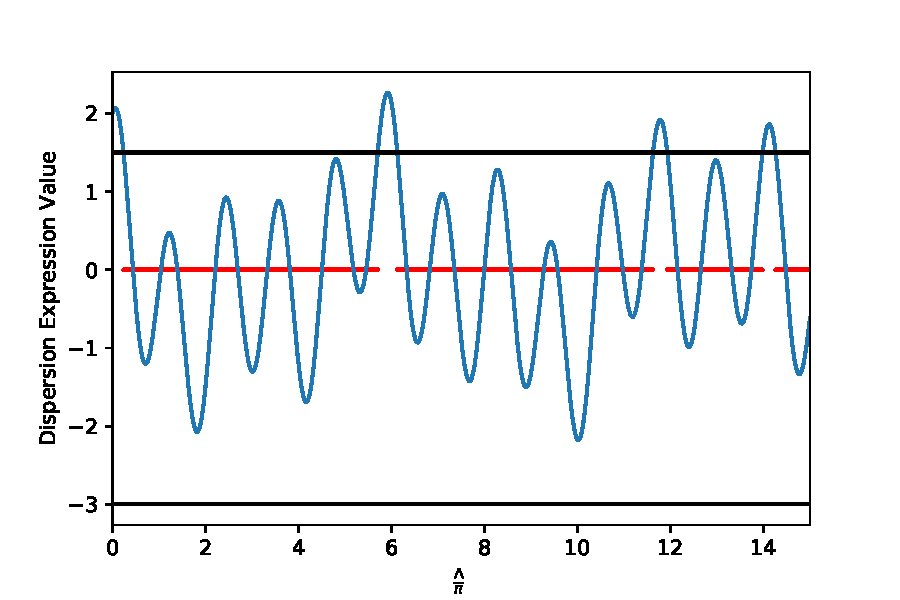
\includegraphics[scale=0.75]{5VertexGraph_SimplifiedLengths_Bandgaps.pdf}
	\caption{\label{fig:5VertexGraph_SimplifiedLengths_Bandgaps} The function $\Xi$ over a range of $\effFreq$. Red regions indicate those $\effFreq$ that correspond to eigenvalues $\omega^2$, when $\Xi\bracs{\effFreq}$ takes values between $-3$ and $\frac{3}{2}$ (black lines). One can see gaps in the spectrum, however we cannot confirm that there are infinitely such many gaps (see text).}
\end{figure}
We can confirm that there exist values $\effFreq$, hence $\omega^2$ that do not correspond to eigenvalues and thus the spectrum of the problem is not the whole real line.
However these are only confirmed numerically, and there is no guarantee that there will be infinitely many such gaps in the spectrum.
Indeed $\Xi$ is not a periodic function of $\effFreq$ (note that the periods of the trigonometric functions are not rational multiples of each other) and so we cannot even plot $\Xi$ over one period in $\effFreq$ and deduce the whole spectrum as in section \ref{sec:ExampleCrossInPlane}.
Thus although we can demonstrate there exist gaps in the spectrum, we cannot guarantee there are infinitely many of them. 
But we can conclude from this example that the geometry alone can be manipulated to give rise to spectral band-gaps, even without the aid of adding coupling constants to our vertices, which is the subject of the example in section \ref{sec:ExampleThickVertex}. \newline

Given the complex expression for $\Xi$; from a practical point of view it would be prudent to probe this system numerically starting from the M-matrix, and solving the generalised eigenvalue problem for eigenvalues over a predetermined range of interest (such as those $\effFreq$ that correspond to typical operating frequencies and wavelengths for fibres).
We have speculated on such a scheme in section \ref{sec:NumericalMethodsDiscussion}; however given that there is no obvious path for analytic progress with this system, we will now turn our attention to another example.

\section{Thick Vertex Case} \label{sec:ExampleThickVertex}
In our final example we look to examine a singular-structure problem which represents (through the equivalent quantum graph problem) the limit of a thin-structure problem in which the vertex- and edge-area scaling is comparable, as discussed in section \ref{sec:GraphLitReview}.
To arrive at such a quantum graph problem from our singular-structure problems in chapter \ref{ch:VectorEqns} we are required to make a slight alteration to the measure we pose our variational problem with respect to.
Specifically we must introduce a point mass at each vertex $v_j$ that is to have a non-zero coupling constant in the equivalent quantum graph problem. 
In general the measure we would be considering in our variational problem would then be $\dddmes$;
\begin{align*}
	\dddmes &= \ddmes + \sum_{v_j\in V}\alpha_j \delta_{j}, \\
	\delta_{j}\bracs{B} &= \begin{cases} 1 & v_j\in B, \\ 0 & v_j\not\in B, \end{cases} \quad\forall B\in\mathcal{B}_{\sqbracs{0,1}^2},
\end{align*}
where the $\alpha_j$ are the coupling constants to appear in the equivalent quantum graph problem (section \ref{sec:DEonQG}), and $\ddmes$ is the singular measure on the underlying (period) graph $\graph$ as defined in section \ref{sec:GraphSingularMeasuresDef}.
Note that the case where $\alpha_j=0 \ \forall v_j\in V$ is the case that was studied in chapter \ref{ch:VectorEqns}, however one can repeat this analysis with respect to this more general measure without too much additional complexity.
This results in the same equations on each edge of $\graph$ (as the $\delta_j$ only have an affect at the vertices) and modified boundary conditions that contain non-zero coupling constants. \newline

For the geometry of this example, we return to the (period graph) defined in section \ref{sec:ExampleCrossInPlane}, and still examine \eqref{eq:QGEquation}.
However we take a non-zero coupling constant $\alpha$ at the vertex $v_3$, meaning that our new boundary conditions are
\begin{align} \label{eq:QGThickVertexConditions}
		u_3 &\text{ is continuous at each } v_j\in V, \\
		0 &= \sum_{j\con k} \bracs{\diff{}{t} + i\qm_{jk}}u_{3,jk}\bracs{v_j}, \quad j\in\clbracs{1,2,4,5}, \\
		\alpha u_3\bracs{v_3} &= \sum_{3\con k} \bracs{\diff{}{t} + i\qm_{3k}}u_{3,3k}\bracs{v_3}.
\end{align}
The $M$-matrix itself is no different to that which we computed in section \ref{sec:ExampleCrossInPlane}, 
\begin{align*}
	M_{\qm}\bracs{\effFreq} &=
	\begin{pmatrix}
		2\effFreq\cot\bracs{\frac{\effFreq}{2}} & 0 & -2\effFreq\csc\bracs{\frac{\effFreq}{2}}\cos\bracs{\frac{\qm_2}{2}} \\
		0 & 2\effFreq\cot\bracs{\frac{\effFreq}{2}} & -2\effFreq\csc\bracs{\frac{\effFreq}{2}}\cos\bracs{\frac{\qm_1}{2}} \\
		-2\effFreq\csc\bracs{\frac{\effFreq}{2}}\cos\bracs{\frac{\qm_2}{2}} & -2\effFreq\csc\bracs{\frac{\effFreq}{2}}\cos\bracs{\frac{\qm_1}{2}} & 4\effFreq\cot\bracs{\frac{\effFreq}{2}}
	\end{pmatrix},
\end{align*}
but now we have a non-zero matrix of coupling constants $A=\mathrm{diag}\bracs{0,0,\alpha}$ and will need to solve
\begin{align*}
	\bracs{M_{\qm}\bracs{\omega^2} - \omega^2 A}v = 0.
\end{align*}
If we chose to proceed numerically we could make use of the suggestion in section \ref{sec:DEonQG} and write $\widetilde{M}_{\qm}\bracs{\omega^2} = M_{\qm}\bracs{\omega^2} - \omega^2 A$; however we will elect to continue our analysis analytically here because it can be shown that
\begin{align*}
	\det\bracs{\bracs{M_{\qm}\bracs{\omega^2} - \omega^2 A}} &= 0 \\
	\Leftrightarrow \cos\bracs{\frac{\qm_1+\qm_2}{2}}\cos\bracs{\frac{\qm_1-\qm_2}{2}} &= \cos\effFreq - \frac{\alpha}{4}\frac{\omega^2}{\effFreq}\sin\effFreq. \labelthis\label{eq:ExampleThickVertexSolution}
\end{align*}
For ease, we define
\begin{align*}
	\Xi\bracs{\omega, \wavenumber} := \cos\effFreq - \frac{\alpha}{4}\frac{\omega^2}{\effFreq}\sin\effFreq.
\end{align*}
As we might expect; there is a lot of similarity between \eqref{eq:ExampleCrossInPlaneSolution} and \eqref{eq:ExampleThickVertexSolution}, the only difference being the introduction of a term with a factor of $\alpha$.
The left hand side of \eqref{eq:ExampleThickVertexSolution} attains every value in the interval $\sqbracs{-1,1}$ over the range $\qm\in[-\pi,\pi)^2$, but the right hand side cannot be written as a function of $\effFreq$ alone.
So finding pairs\footnote{We could elect to find pairs $\bracs{\omega, \effFreq}$ of course; but as $\effFreq$ is a function of $\omega$ and $\wavenumber$, and the conventions that surround dispersion relations, it makes more sense to phrase things in terms of $\bracs{\omega, \wavenumber}$.} $\bracs{\omega, \wavenumber}$ amounts to finding all $\bracs{\omega, \wavenumber}$ such that
\begin{align} \label{eq:ExampleThickVertexDispExpr}
	-1 \leq \Xi\bracs{\omega, \wavenumber} \leq 1.
\end{align}
One can visualise the curve $\Xi$ for a fixed value of $\wavenumber=\pi$ (and with $\alpha=-1$) in figure \ref{fig:ThickVertex_CurlsTFRSetup_k1a1}.
\begin{figure}[t]
	\centering
	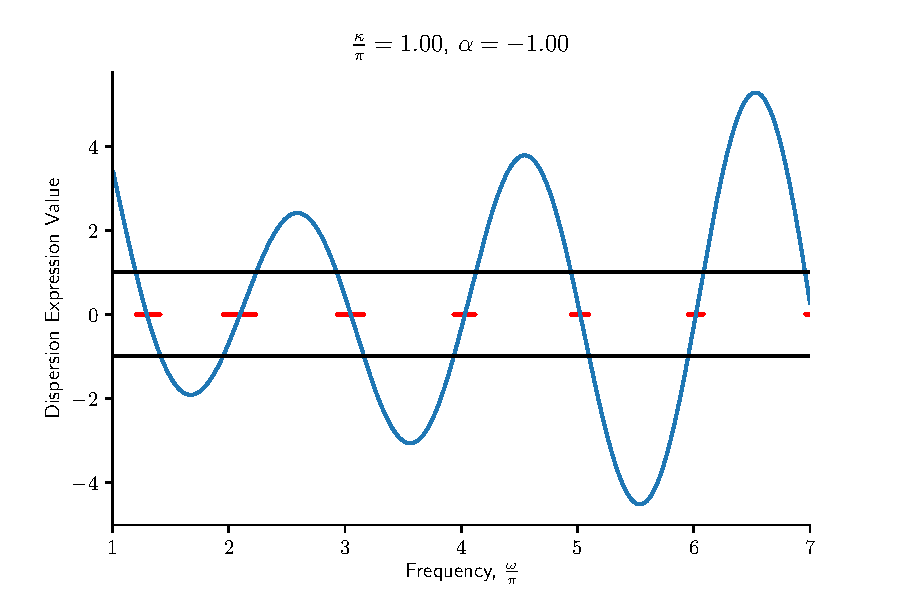
\includegraphics[scale=0.75]{ThickVertex_CurlsTFRSetup_k1a1.pdf}
	\caption{\label{fig:ThickVertex_CurlsTFRSetup_k1a1} The function $\Xi$ for a fixed value of $\wavenumber=\pi$. Red regions indicate those $\omega$ that correspond to eigenvalues $\omega^2$, when $\Xi\bracs{\omega, \pi}$ takes values between $-1$ and $1$ (black lines). One can see the existence of spectral bands which shrink in size as $\omega\rightarrow\infty$.}
\end{figure}
We can observe that for a fixed $\wavenumber$ the points $\omega$ that satisfy \eqref{eq:ExampleThickVertexDispExpr} are divided into distinct ``spectral bands" which shrink as $\omega\rightarrow\infty$.
Of course the value of $\alpha$ changes the shape of $\Xi$ which in turn will also effect the set of points $\bracs{\omega, \wavenumber}$ that solve \eqref{eq:ExampleThickVertexDispExpr}. \newline

Of course, of greater physical significance is the band-gap-plot that \eqref{eq:ExampleThickVertexDispExpr} gives rise to, as presented in figure \ref{fig:ThickVertex_CurlsTFRSetup}.
\begin{figure}[b!]
	\centering
	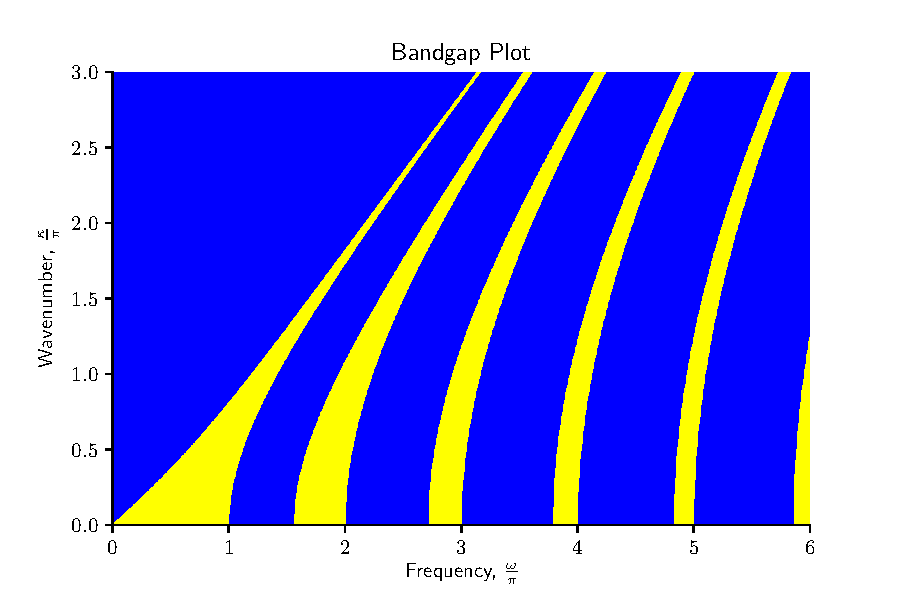
\includegraphics[scale=0.75]{ThickVertex_CurlsTFRSetup.pdf}
	\caption{\label{fig:ThickVertex_CurlsTFRSetup} Dispersion plot for the system in section \ref{sec:ExampleThickVertex}, yellow regions correspond to $\omega, \wavenumber$ pairs that solve \eqref{eq:CurlCurlEquationDivFree}. We observe spectral ``band-gaps" in $\omega$ for each $\wavenumber$, with the same basic shape as those from fabricated PCFs, although lacking some specific features of these plots.}
\end{figure}
In this figure points $\bracs{\omega, \wavenumber}$ in yellow correspond to solutions to \eqref{eq:ExampleThickVertexDispExpr}, whilst those in blue do not.
Here we see that there are distinct branches or regions of $\bracs{\omega, \wavenumber}$ in which we obtain solutions to \eqref{eq:QGEquation} with \eqref{eq:QGThickVertexConditions} as the boundary conditions.
Importantly the shape of these regions is similar to experimental band-gap plots in a PCF setting, displaying bands that shrink in width as $\wavenumber$ increases in number.
This should not be unexpected, but also should be interpreted cautiously, our singular-structure problem has recreated the basic shape of a band-gap plot, but lacks several features of experimental plots - notably the possibility of band-gaps merging as $\wavenumber$ increases or terminating (like at the tip f a spike) at some finite $\bracs{\omega, \wavenumber}$ values.
Recovery of these features may be outside the scope of the curl-of-the-curl equation \eqref{eq:CurlCurlEquationDivFree}, and we may require a more general system of starting equations to capture this behaviour (section \ref{sec:ConcFutureMaxwell}).

\section{Chapter Summary} \label{sec:ExamplesSummary}
The examples in this chapter demonstrate how we can determine the spectrum of singular-structure problems, bringing together the theory of chapters \ref{ch:QuantumGraphs} and \ref{ch:VectorEqns}, and also highlight several issues that need to be considered during the solution process.
Of particular note is the central role that the M-matrix plays in our computations, and how it can be easily constructed by proposition \ref{prop:M-MatrixEntries}.
Of course, one still needs to find an analogue of proposition \ref{prop:M-MatrixEntries} for every quantum graph problem they want to solve in this manner.
Combined with the fact that determining the spectrum of our singular-structure problems amounts to solving a generalised eigenvalue problem, this provides us with a (albeit na\"ive) numerical method for situations when analytic progress proves difficult.
We have speculated on some of the issues such a numerical scheme would face in section \ref{sec:NumericalMethodsDiscussion}, and will revisit this idea of developing a suitable numerical scheme for handling these problems in chapter \ref{ch:Conclusion}. \newline

The examples that we consider in sections \ref{sec:ExampleCrossInPlane} and \ref{sec:ExampleGeneralLengths} are chosen so as to demonstrate that analytic progress is possible for small graphs with simple geometries; but unless our system exhibits a great deal of symmetry we are often forced to resort to numerical techniques to investigate the spectrum.
Section \ref{sec:ExampleCrossInPlane} gives an example of a problem whose spectrum can be determined analytically; although this spectrum turns out to be rather uninteresting from a wave-guidance viewpoint, as it doesn't exhibit band-gaps.
It does provide a concrete example as to how we go about determining the spectrum of our singular-structure problems though, and illustrates the utility of the M-matrix in storing all the information we need about our problem to reach an understanding of it's spectrum.
The example in section \ref{sec:ExampleGeneralLengths} illustrates how introducing slight complexities and breaking symmetries in the underlying geometry makes analytic progress difficult, but not impossible.
Pursuing an analytic approach yields an expression for the spectrum that is difficult to treat, although some numerical investigations do confirm the existence of band-gaps in the spectrum.
Whether there are infinitely many spectral bands however is still an open question, and would require a detailed analysis of \eqref{eq:5VertexGraphDispExpr} - at present all that has been carried out is an investigation into a single, rather simplified, case.
From a fibre-design perspective, a numerical scheme that begins from the M-matrix would be beneficial here because of the complexity of the resulting analytic expressions.
Such a scheme could be used to investigate the spectrum at specific ranges of interest (for example, near operating frequencies for fibres), which bypasses the need to determine the complete spectrum. \newline

In section \ref{sec:ExampleThickVertex} we explored an example quantum graph problem with non-zero coupling constants at the central vertices.
This quantum graph problem represents the limit of a family of thin-structure problems with the thickness of the structure scaling in a different way to the previous examples, as discussed in section \ref{sec:GraphLitReview}.
Also provided was the singular-structure problem that we would begin from to obtain this quantum graph problem as an equivalent formulation, following much the same analysis as in chapter \ref{ch:VectorEqns} but with slightly altered measures in our variational formulation.
This example used the same geometry as the example of section \ref{sec:ExampleCrossInPlane}, however due to the presence of a non-zero coupling constant at the central vertex we observe spectral band-gaps in $\omega$ at all values of $\wavenumber$.
The dispersion plot that we can produce from our analysis also bears some base-level resemblance in it's shape to experimentally-determined dispersion plots for band-gap fibres.
This would imply that a specific scaling between the vertex- and edge-areas results in ``easier" opening of band-gaps in PCFs, although formal investigation needs to be carried out to validate this hypothesis.
Also worthy of note in this example is that the M-matrix remains the same as that in section \ref{sec:ExampleCrossInPlane}, the only difference being that we have a non-zero matrix of coupling constants to handle.
Again coming from a numerical viewpoint; this means that investigating the same geometries but with different vertex conditions will only require construction of (a function that evaluates) the M-matrix once, but the coupling constants in the quantum graph problem can then be readily changed without a need to rebuild the M-matrix. \newline

In chapter \ref{ch:Conclusion} we will discuss some of the key concepts that we have developed in this report, and revisit some of the ideas highlighted by the examples in this section.
We will also revisit the motivation of chapter \ref{ch:Intro} and reiterate the link between the work we have done here and the application it has to wave-guidance in PCFs, as well as speculate on the direction of future work.